\documentclass[12pt,border=0pt]{standalone}

\usepackage[utf8]{inputenc} 
\usepackage{amssymb,amsmath}
\usepackage{tikz}
\usetikzlibrary{positioning}


\thispagestyle{empty}

\begin{document}

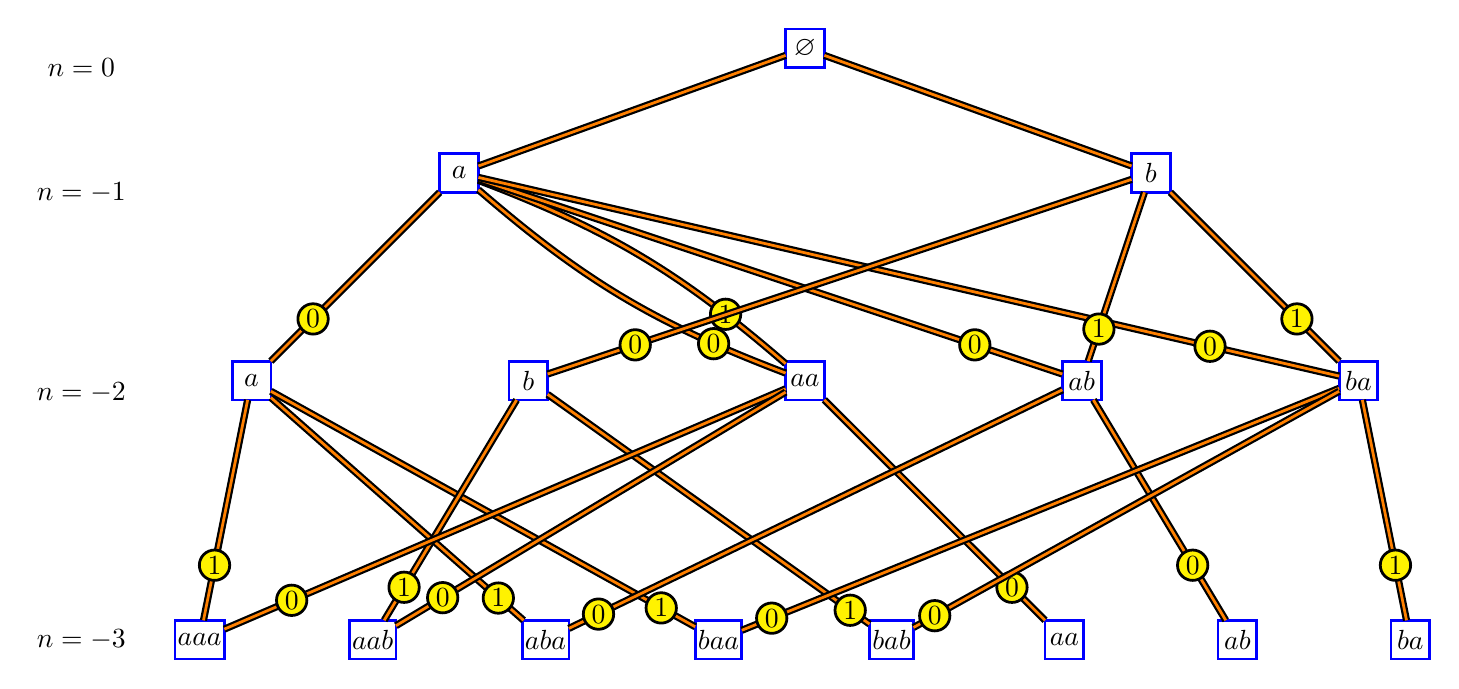
\begin{tikzpicture}[x=10pt,y=6pt]
  \centering
  \tikzset{VertexStyle/.style = {
    shape         = rectangle,
    draw          = blue, 
    fill          = white, 
  	line width    = 1pt, 
    text          = black,
    inner sep     = 1pt,
    outer sep     = 0pt,
    minimum size  = 14 pt,
    scale         = 1
    }
  }
  \tikzset{EdgeStyle/.style = {
    draw            = black, 
    thick,
    double          = orange,
    double distance = 1pt
    }
  }
  \tikzset{EdgeLabelStyle/.style = {
    draw          = black,
  	shape         = circle, 
  	line width    = 1pt, 
  	minimum size  = 10pt, 
    inner sep     = 1pt,
    outer sep     = 0pt,
    fill          = yellow,
    text          = black,
    scale         = 1
    }
  }

	\node[VertexStyle](A1) at (25, 38.75) {$\varnothing$};
	\node[VertexStyle](B1) at (12.5, 31.25) {$a$};
	\node[VertexStyle](B2) at (37.5, 31.25) {$b$};
	\node[VertexStyle](C1) at (5, 18.75) {$a$};
	\node[VertexStyle](C2) at (15, 18.75) {$b$};
	\node[VertexStyle](C3) at (25, 18.75) {$aa$};
	\node[VertexStyle](C4) at (35, 18.75) {$ab$};
	\node[VertexStyle](C5) at (45, 18.75) {$ba$};
	\node[VertexStyle](D1) at (3.125, 3.141) {$aaa$};
	\node[VertexStyle](D2) at (9.375, 3.141) {$aab$};
	\node[VertexStyle](D3) at (15.625, 3.141) {$aba$};
	\node[VertexStyle](D4) at (21.875, 3.141) {$baa$};
	\node[VertexStyle](D5) at (28.125, 3.141) {$bab$};
	\node[VertexStyle](D6) at (34.375, 3.141) {$aa$};
	\node[VertexStyle](D7) at (40.625, 3.141) {$ab$};
	\node[VertexStyle](D8) at (46.875, 3.141) {$ba$};
	\draw[EdgeStyle](A1) to (B1);
	\draw[EdgeStyle](A1) to (B2);
	\draw[EdgeStyle](B1) to node[EdgeLabelStyle, pos=0.75]{$0$} (C1);
	\draw[EdgeStyle, bend left=-10, pos=0.8](B1) to node[EdgeLabelStyle]{$0$} (C3);
	\draw[EdgeStyle, bend left=10, pos=0.8](B1) to node[EdgeLabelStyle]{$1$} (C3);
	\draw[EdgeStyle](B1) to node[EdgeLabelStyle, pos=0.85]{$0$} (C4);
	\draw[EdgeStyle](B1) to node[EdgeLabelStyle, pos=0.85]{$0$} (C5);
	\draw[EdgeStyle](B2) to node[EdgeLabelStyle, pos=0.85]{$0$} (C2);
	\draw[EdgeStyle](B2) to node[EdgeLabelStyle, pos=0.81]{$1$} (C4);
	\draw[EdgeStyle](B2) to node[EdgeLabelStyle, pos=0.75]{$1$} (C5);
	\draw[EdgeStyle](C1) to node[EdgeLabelStyle, pos=0.75]{$1$} (D1);
	\draw[EdgeStyle](C1) to node[EdgeLabelStyle, pos=0.9]{$1$} (D3);
	\draw[EdgeStyle](C1) to node[EdgeLabelStyle, pos=0.92]{$1$} (D4);
	\draw[EdgeStyle](C2) to node[EdgeLabelStyle, pos=0.85]{$1$} (D2);
	\draw[EdgeStyle](C2) to node[EdgeLabelStyle, pos=0.94]{$1$} (D5);
	\draw[EdgeStyle](C3) to node[EdgeLabelStyle, pos=0.88]{$0$} (D1);
	\draw[EdgeStyle](C3) to node[EdgeLabelStyle, pos=0.88]{$0$} (D2);
	\draw[EdgeStyle](C3) to node[EdgeLabelStyle, pos=0.85]{$0$} (D6);
	\draw[EdgeStyle](C4) to node[EdgeLabelStyle, pos=0.94]{$0$} (D3);
	\draw[EdgeStyle](C4) to node[EdgeLabelStyle, pos=0.75]{$0$} (D7);
	\draw[EdgeStyle](C5) to node[EdgeLabelStyle, pos=0.95]{$0$} (D4);
	\draw[EdgeStyle](C5) to node[EdgeLabelStyle, pos=0.95]{$0$} (D5);
	\draw[EdgeStyle](C5) to node[EdgeLabelStyle, pos=0.75]{$1$} (D8);

	\node[left=0.5cm of D1](n3){$n=-3$};
	\node[above=75pt of n3](n2){$n=-2$};
	\node[above=58pt of n2](n1){$n=-1$};
	\node[above=31pt of n1]{$n=0$};
  \end{tikzpicture}

\end{document}
